
\chapter{On the Computation of Transonic Flows}\label{chap6}%chap 6
 
\section{Introduction}\label{c6:s1}%sec 1.
We have\pageoriginale considered in Chapter~\ref{chap4},
Section~\ref{c4:s3},  the  
non-linear elliptic equation describing the \textit{subsonic flows} of 
an \textit{inviscid compressible fluid.}   

In this chapter, following closely GLOWINSKI - PIRONNEAU
[\ref{k55:e1}],  we would  
 like to give some brief indications on the  computation of transonic 
 flows for similar fluids.  Given the importance and the complexity of 
 the problem to be described in a moment, we would  like to point out 
 that the following considerations are just an introduction to the 
 subject and that many methods,  using very different approaches,  
 exist in the specialized literature (see the following  references ).  
 Moreover,  we would like to mention that from a mathematical point of 
 view,  the methods to be described in the following sections are 
 widely heuristical.  A large number of bibliographical references are 
 given in the sequel.           

\section{Generalities}\label{c6:s2}

The theoretical and numerical studies of \textit{transonic flows for 
inviscid fluids} have always been very important questions.  But these 
problems have become even more important in recent years in relation to 
the design and development of \textit{large subsonic economical 
aircrafts}.    

From the theoretical point of view a lot of open questions still 
remains, with their counterparts in the numerical methodology. The  
difficulties are quite considerable for the following reasons:   
\begin{enumerate}[(1)]
\item The problems are \textit{nonlinear};
\item \textit{Shocks} may exist in the flow;
\item One has to include an \textit{entropy conditions}, in one way or 
another, to avoid non-physical solutions.  
\end{enumerate}
From the\pageoriginale \textit{theoretical} point of view we have to
mention the work  
of BERS [\ref{k11:e1}], C. MORAVETZ [\ref{k70:e1}]. At  the present
moment the more commonly  
used  numerical methods have originated from MURMAN-COLE
[\ref{k72:e1}] and we  
shall mention BAUER-GARABEDIAN-KORN [\ref{k4:e1}],  BAUER-GARABEDIAN - KORN 
JAMESON [\ref{k5:e1}],  JAMESON [\ref{k59:e1}], [\ref{k59:e2}],
[\ref{k59:e3}], [\ref{k59:e4}] and the bibliographies therein  
(see also HEWITT-ILLINGWORTH and co-editors [\ref{k56:e1}]).      

These above numerical methods use the key idea of Murman and Cole which 
consists in the use of a \textit{finite difference scheme, centered} in 
the  \textit{subsonic} part of the flow,  \textit{backward} (in the 
direction of the flow) in the \textit{supersonic part}. The switching 
between these two schemes is automatically done via $a$ 
\textit{truncation operator} only active in the \textit{supersonic} 
part of the flow (see JAMESON, loc. cit., for more details). A 
\textit{relaxation} method is then used to solve the resulting 
nonlinear system (actually, \textit{over-relaxation} is used in the 
subsonic part of the flow, \textit{under-relaxation} in the supersonic 
part).           

We shall describe a different approach -very convenient for 
\textit{nozzles,  and flows subsonic at infinity around airfoils} - in 
which the transonic flow problem is formulated as a \textit{nonlinear 
least square problem}.  This  last problem is then viewed as an 
\textit{optimal control problem} which  is approximated by a 
\textit{finite element} method.  Since the entropy  condition is 
formulated by a \textit{linear inequality constraint}, a convenient 
method to handle it is to use \textit{penalty} and/or \textit{duality} 
methods (see CEA [\ref{k27:e1}], [\ref{k27:e2}]),  using an
\textit{augmented Lagrangian} if  
penalty and duality are combined. Then the approximate problem is 
solved by \textit{iterations} of \textit{conjugate gradient} type.  Our 
approach is strongly  motivated by the two following points of view and 
the corresponding  methodologies:              
\begin{enumerate}[(1)]
 \item \textit{Optimal control of distributed parameter system }(see 
 LIONS [\ref{k67:e4}], CEA [\ref{k27:e1}], [\ref{k27:e2}]),   
 \item \textit{Variational inequalities and their numerical  solution} 
 (see  GLOWI\-NSKI-LION-TREMOLIERES [\ref{k53:e1}], [\ref{k53:e2}],
   [\ref{k53:e3}] and Chapters 1 to 5 of these notes).   
\end{enumerate}

\section[Mathematical Model For The Transonic...]{Mathematical Model
  For The Transonic\hfil\break Flow Problem}\label{c6:s3} %sec 3. 

\subsection{Basic assumptions and generalities}\label{c6:ss3.1}%sub sec 3.1.

We assume\pageoriginale that the fluid under consideration is
\textit{inviscid} and  
\textit{compressible} and that the flow of such a fluid is 
\textit{is entropic} and \textit{irrotational} (i.e. 
\textit{potential)}.  These assumptions are not true in general,  since 
through a shock there is a \textit{variation of entropy} and an 
\textit{irrotational flow becomes rotational}; therefore the validity 
of the model to follow is assumed to be correct only in the case of a 
\textit{``weak shock''}.        

In the case of a flow past a \textit{sharp airfoil} we shall suppose 
that there is \textit{no wake behind the trailing edge}.  

\subsection{Equations of the flow}\label{c6:ss3.2}%sub sec 3.2
Let $\Omega$ be the domain of the flow and $\Gamma$ its boundary; then 
the flow is modelled by  
\begin{equation}
-\nabla \left( \left( 1 - \frac{|\nabla \Phi 
|^2}{\frac{\gamma + 1}{\gamma - 1}C^2_*}\right)^{\frac{1}{\gamma - 
1}}\nabla \Phi \right) = 0 \text{ in }\Omega, \tag{3.1}\label{c6:eq3.1}  
\end{equation}
where 
\begin{enumerate}[-]
\item $\Phi$  is  the \textit{flow potential}, $\nabla \Phi$  
the \textit{flow velocity},  
\item $C_*$ is the \textit{critical velocity, }
\item $\gamma$ is the ratio of specific heats $( \gamma =$ 1. 4 for air).  
\end{enumerate}
We have to add to\eqref{c6:eq3.1} 
\begin{itemize}
\item Boundary conditions (of Dirichlet and/or Neumann type,  for example);
\item \textit{Kutta-Joukowsky} condition in the case of the flow
  around a lifting body (see LANDAU - LIFCHITZ [\ref{k64:e1},  Sec. 46]); some
  indications are also given in Sec. 5.1,  Remark 5. 1. 
\item An \textit{entropy condition} in order to eliminate the 
non-physical solutions of \eqref{c6:eq3.1}; this point will be 
discussed in Sec. 3.3   
\end{itemize}

\begin{remark}\label{c6:rem3.1} %remark 3. 1
 It can happen that on some part of the boundary,  $\Phi $ and 
 $\dfrac{\partial \Phi}{\partial n}$  have to be given 
 \textit{simultaneously }  to ensure uniqueness; it is the case, for 
 instance, for the \textit{divergent} nozzle of Figure 3.1 if the 
 velocity  at the entrance is \textit{supersonic}. Typical boundary 
 conditions are $\Phi$ given on $\Gamma_1$, $\Gamma_3$ and 
 $\dfrac{\partial \Phi}{\partial n}$ given on $\Gamma_4$, $\Gamma_1$, 
 $\Gamma_2$; if the flow at the entrance (i.e.  $\Gamma_1$) is 
 \textit{subsonic} we require \textit{fewer} boundary conditions.       
 \end{remark}

\begin{figure}[H]
\centering{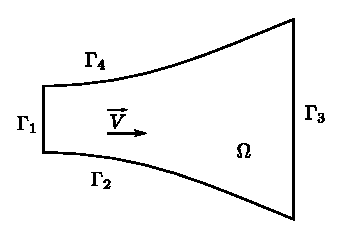
\includegraphics{vol65-figures/fig65-chap3.1_1.eps}}
\caption{}\label{c6:fig3.1}
\end{figure}

\begin{figure}[H]
\centering{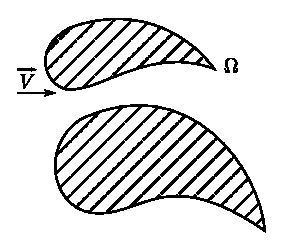
\includegraphics{vol65-figures/fig65-chap3.2_1.eps}}
\caption{}\label{c6:fig3.2}
\end{figure}


\begin{remark}\label{c6:rem3.2}%remark 3. 2
In the\pageoriginale  case of the flow around a multipiece airfoil,  (like in 
Fig. \ref{c6:fig3.2} \textit{each} piece requires a Kutta-Joukowsky condition.  
\end{remark} 
 
\begin{exercise}\label{c6:exer3.1}%exercise 3. 1 
Verify that \eqref{c6:eq3.1} is elliptic if $| \nabla \phi| < C_* 
$ (\textit{subsonic} zone),  hyperbolic if $| \nabla \phi | > 
C_*$ (\textit{supersonic} zone).    
 \end{exercise} 
 
 \subsection{Formulation of the entropy condition}\label{c6:ss3.3}

 It follows from  LANDAU-LIFCHITZ [\ref{k64:e1}, Ch. 9] that the
 \textit{entropy condition} can be formulated as follows   
 \begin{equation}
\begin{cases}
\text{In the direction of the flow,  once cannot have a subsonic-}\\
\text{supersonic transition through a shock.} \tag{3.2}\label{c6:eq3.2}
\end{cases} 
 \end{equation} 
 For \textit{one dimensional } flow,  \eqref{c6:eq3.2} implies 
 \begin{equation}
\frac{d^2 \Phi}{dx^2}< + \infty, \tag{3.3}\label{c6:eq3.3}
 \end{equation} 
 i. e.  $\dfrac{d^2 \Phi}{dx^2}$ is a \textit{measure bounded from 
 above; weak}(and more precise) formulations  of \eqref{c6:eq3.3} are : 
 \textit{There exists a constant $M$,  such that either}  
 \begin{equation}
-\int_\Omega \frac{d \Phi}{dx} \frac{d \phi}{dx} dx \leq M \int_\Omega 
\phi dx\quad  \forall \phi \in \mathscr{D}_+ (\Omega 
)\tag{3.4}\label{c6:eq3.4}   
 \end{equation} 
 \textit{or}
 \begin{equation}
\int_\Omega \phi \frac{d^2 \phi}{dx^2}dx \leq M \int_\Omega dx  \quad 
\forall \phi \in  \mathscr{D}_+ (\Omega )\tag{3.5}\label{c6:eq3.5} 
\end{equation} 
 where
\begin{equation}
\mathscr{D}_+ (\Omega ) = \{ \phi \in \mathscr{D} (\Omega ), \phi 
\geq 0 \}. \tag{3.6}\label{c6:eq3.6}  
\end{equation}\pageoriginale 
In the case of a \textit{two or three dimensional flow}, we shall 
suppose that \eqref{c6:eq3.2} can be formulated as  
\begin{equation}
\triangle \Phi < + \infty \tag{3.7}\label{c6:eq3.7}
\end{equation}
or in a \textit {weak from} either by
\begin{equation}
 -\int_\Omega \nabla \Phi \cdot \nabla \phi dx \leq M 
 \int_\Omega \phi dx \, \forall \phi \in \mathscr{D}_+ (\Omega 
 ) \tag{3.8}\label{c6:eq3.8}
\end{equation}
or by
\begin{equation}
\int_\Omega \Phi \triangle \phi dx \leq M \int_\Omega \phi dx \quad 
\forall \phi \in \mathscr{D}_+ (\Omega ). \tag{3.9}\label{c6:eq3.9}
\end{equation}
The numerical results that we have obtained for \textit 
{two-dimensional} flows, using discrete analogs  of \eqref{c6:eq3.7}, 
seem to justify the above formulations of the entropy condition.  

\section{Reduction to an Optimal Control Problem}

If we suppose that the density on the fluid is on if $\uu\limits_\sim 
= \nabla \Phi = 0$, then the coefficient of $\nabla \Phi$ in 
\eqref{c6:eq3.1} appears as the \textit {density} of the fluid. We 
shall use the notation   
\begin{equation}
\rho (\phi ) = \left( 1 -\frac{|\nabla \phi |^2} {\frac{\gamma + 
1} {\gamma - 1}} C^2_*\right)^{\frac{1}{\gamma - 1}} 
\end{equation}
The idea of the method to follows, is to \textit {decouple} the density 
and the potential $\Phi$. To do so we introduce a new potential $\xi$ 
-the control potential -and try to recouple $\xi$ and $\Phi$ by 
minimizing some \textit {cost function} of \textit {least square type}. 
We may use for instance the following formulation (for the formulation 
see BRISTEAU [\ref{k21:e2}], BRISTEAU - GLOWINSKI - PERIAUX - PERRIER
- PIRONNEAU  
[\ref{k23:e1}], BRISTEAU - GLOWINSKI - PERIAUX - PERRIER - PIRONNEAU - POIRIER 
[\ref{k24:e1}])       
\begin{equation}
\min_\xi \int_\Omega \rho^\alpha (\xi ) | \nabla (\Phi -\xi )|^2 
dx , \xi \in X \tag{4.2}\label{c6:eq4.2} 
\end{equation}
where, in \eqref{c6:eq4.2} $\Phi$ is a function of $\xi$ via the 
\textit{state equation} 
\begin{equation}
\begin{cases}
- \nabla \cdot (\rho (\xi ) \nabla \Phi ) = 0 \text{ over 
} \Omega \\ 
+ \text{ boundary conditions for } \Phi \text{ on } \Gamma.  
\end{cases}
\tag{4.3}\label{c6:eq4.3}
\end{equation}\pageoriginale 
In \eqref{c6:eq4.2} the parameter $\alpha$ is either 0 of 1 and $X$ is 
a \textit{convex} set ``conveniently'' chosen. Since $\rho (\phi (x) ) 
= 0$ iff $|\nabla \phi (x) | = \left( \frac{\gamma + 1}{\gamma 
- 1} \right)^{1/2} C_*$, and that for \textit{air} we have $\gamma = 1. 
4$ which implies $\left( \frac{\gamma + 1}{\gamma -1}\right)^{1/2} = 
\sqrt{6} \simeq 2. 45$, it appears that in the transonic range (say $| 
\vec{v}| = | \nabla \phi | \leq 1. 5 C_* $) we have        
\begin{equation}
0 < \delta < \rho (\phi (x)) \leq 1 a.e. \text{ on } \Omega. 
\tag{4.4}\label{c6:eq4.4} 
\end{equation}
it follows from \eqref{c6:eq4.4} that \eqref{c6:eq4.3} is an 
\textit{elliptic problem} for appropriate boundary conditions. In the 
case of flows around lifting airfoils, \textit{Kutta-Joukowsky 
conditions} are also required in order to obtain, with the other 
boundary conditions, a physical solution  of problem \eqref{c6:eq4.3} 
(modulo a constant if one has only Neumann conditions on the boundary).  
     

\begin{remark}\label{c6:rem4.1}% remark 4.1
If in the original problem, $\Phi$ and $\dfrac{\partial \Phi}{\partial 
n}$ have to be simultaneously prescribed on some part of $\Gamma$, the 
previous approach with two- potentials is very convenient since the 
boundary conditions can be split between $\Phi$ and $\xi$. However, if 
one wishes to use the same boundary conditions for $\Phi$ and $\xi$ it 
is always possible to take into account the extra boundary conditions 
(assumed to be of Dirichlet type) by adding to the cost function 
\eqref{c6:eq4.2} a quantity proportional to either 
$\int_{\Gamma_d}|\Phi - \Phi_d|^2 d \Gamma$, or $\int_{\Gamma_d}| 
\Phi- \Phi_d |^2$ (or to a linear combination of both), where 
$\Gamma_d$ is the part of $\Gamma$ where one requires $\Phi 
|_{\Gamma_d} = \Phi_d$. A similar idea is used in BEGIS-GLOWINSKI [2] 
to solve some free boundary problem.            
\end{remark}

\begin{remark}\label{c6:rem4.2}% remark 4.2
To state the entropy {\em conditions} \eqref{c6:eq3.7} (or its weak 
formulations \eqref{c6:eq3.8}, (\ref{c6:eq3.9})) we have the choice 
between $\Phi$ and $\xi$ (actually we can also use these two potentials 
simultaneously). If one uses $\xi$ (resp. $\Phi $) we have a {\em 
constraint on the control} (resp. {\em constraint on the state}).     
\end{remark}

\begin{remark}\label{c6:rem4.3}%remark 4. 3
We observe that the class of flows we are considering, is physically 
such that  
$$
|| \vec{v} ||_\infty = || \nabla \Phi ||_\infty < + \infty.
$$
It follows\pageoriginale  from this remark that the convex set occurring in 
\eqref{c6:eq4.2} will be taken as a convex subset of $W^{1, \infty} 
(\Omega )$. We observe also that to stay in the transonic range it may 
be convenient to introduce following constraints (if $\gamma = 1. 4$):  
\begin{equation}
|\nabla \xi | \leq v_M < \sqrt{6} C_* \tag{4.5}\label{c6:eq4.5}
\end{equation}
or 
\begin{equation}
|\nabla \Phi | \leq v_M < \sqrt{6} C_*. \tag{4.6}\label{c6:eq4.6}
\end{equation}
Actually, the computations we have done proved that for a 
\textit{physically} well - posed travsonic problem it is not necessary 
to introduce \eqref{c6:eq4.5} or \eqref{c6:eq4.6}.  
\end{remark}

\begin{remark}\label{c6:rem4.4}%remark 4.4
If the transonic problem has a solution and if $X$ is ``large enough'' 
the control problem will have a solution such that the {\em cost 
function will be equal to zero}; this last property will give us (for 
the approximate problem) indications to check the quality of the 
computed solution.     
\end{remark}

\section{Approximation}\label{c6:s5}%sec 5.

We assume that $\Omega \subset \mathds{R}^2$.

\subsection{Generalities}\label{c6:ss5.1} 
The above control problem will be approximated by a \textit{finite 
element method}, since compared to \textit{finite difference} methods 
it give us the possibility of handling problems posed on rather 
complicated geometry. Moreover the \textit{variational foundations} of 
finite element formulations are very appropriate to the problem under 
consideration. It will be in particular easy to approximate the weak 
formulations of the entropy condition \eqref{c6:eq3.7}.       

If $\Omega$ is \textit{unbounded} it will be replaced by a 
\textit{bounded domain} - still denoted by $\Omega$- as large as 
possible.  To approximate the above continuous problems we introduce a 
standard \textit{triangulation} $\mathscr{C}_h$ of $\Omega$ (we can also use 
\textit{quadrilateral finite elements} defined over a 
``quadrangulation'' of $\Omega$). Then the functions $\xi$ and $\Phi$ 
are approximated by piecewise polynomial functions belonging to the 
following subspace $V_h $ of $H^1 (\Omega )$.       
\begin{equation}
V_h = \left\{ \Phi_h \in C^0 (\overline{\Omega}), \Phi_h |_T \in 
P_k \forall T \in \mathscr{C}_h \right\}, \tag{5.1}\label{c6:eq5.1}  
\end{equation}
with $P_k = $ the space of polynomials of degree $\leq k$. 

\begin{remark}\label{c6:rem5.1}%remark 5.1
In the\pageoriginale  case of a {\em lifting body}, to take into account the {\em 
Kutta - Joukowsky condition}, one usually introduces (see Fig. \ref{c6:fig5.1})  an 
arc $\gamma$ between the leading edge of the profile and the external 
boundary. This arc $\gamma$ supports a {\em constant jump (a priori 
unknown)} of $\Phi$ (and $\xi$) and this jump has to be adjusted in 
such a way that $\dfrac{\partial \Phi}{\partial n}$ (and 
$\dfrac{\partial \xi}{\partial n}$) is ``continuous'' when crossing 
$\gamma$. Since $\Phi$ is discontinuous along $\gamma$, we cannot work 
anymore with $H^1 (\Omega )$, but introducing $\dot{\Omega} =$ 
$\displaystyle{\mathop{\circ}_{\overline{\overline{\Omega} -
      \gamma}}}$ one can use $H^1 (\dot{\Omega})$  
and define $V_h$ over a triangulation of $\Omega$.           
\end{remark}

In Sec.~\ref{c6:s7}, results of computations for such airfoils are 
given; however for the sake of simplicity the numerical treatment of 
the Kutta-Joukowsky condition will not be discussed here and we shall 
assume in the sequel that one works directly over $\Omega$.    

\begin{remark}\label{c6:rem5.2}% remark 5.2
If $\Phi$ and $\xi$ have to satisfy only {\em Neumann boundary 
conditions}, the subspace of $V_h$ to be used will be $V_h$ itself. On 
the contrary if $\Phi$ and /or $\xi$ have satisfy {\em Dirichlet 
boundary conditions} somewhere over $\Gamma $ then we shall have to use 
subspaces of $V_h$ {\em strictly} included in $V_h$.    
\setcounter{figure}{0}
\begin{figure}[H]
\centering{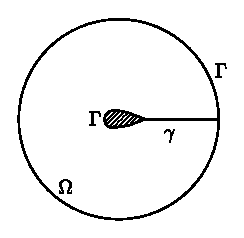
\includegraphics{vol65-figures/fig65-chap5.1_1.eps}}
\caption{}\label{c6:fig5.1}
\end{figure}
\end{remark}

\begin{remark}\label{c6:rem5.3}%remark 5. 3
We have tacitly assumed that $\Omega$ is a polygonal domain of 
$\mathds{R}^2$ or has been approximated by such a domain. However in 
the case of a curved boundary, it is always possible to use (at some 
extra computational cost) {\em curved finite elements} (See, for 
instance CIARLET-RAVIART [\ref{k32:e1}], STRANG - FIX [\ref{k85:e1},
  Ch. 3], CIARLET [\ref{k31:e1}], [\ref{k31:e3}]).     
\end{remark}

\begin{remark}\label{c6:rem5.4}% remark 5.4
It follows from \eqref{c6:eq5.1} that we are using {\em $C^0$ - 
conforming} finite elements. Since the regularity of the solution is 
limited it seems that it would be unrealistic to use $k \geq 3$. 
Therefore only {\em Lagrange elements} will be considered. One may also 
use that non $C^0$- conforming element of Figure~\ref{c6:fig5.2} in which, with 
$\phi_{h | T}\in P_1$, one only requires the continuity of $\phi_h$ 
at the mid-point of each side of the $T \in \mathscr{C}_h$. The 
number of unknowns, when using this element is much in higher than when 
using \eqref{c6:eq5.1} with $k = 1$.        
\end{remark}

\begin{figure}[H]
\centering{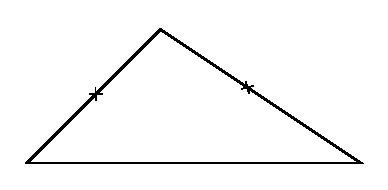
\includegraphics{vol65-figures/fig65-chap5.2.eps}}
\caption{}\label{c6:fig5.2}
\end{figure}

\subsection{Approximation of the state equation and of the cost 
function}\label{c6:ss5.2}%5. 2.

To simplify\pageoriginale  the presentation we shall assume that we only have 
\textit{Neumann boundary conditions} i.e.  
\begin{equation}
\frac{\partial \Phi}{\partial n} = g \text{ on } \Gamma 
\tag{5.2}\label{c6:eq5.2} 
\end{equation}
(it is the case for the very important application of flows around 
airfoils, \textit{subsonic at infinity}). It follows from the above 
sections that we can take the \textit{same boundary conditions} for 
$\xi$ and $\Phi$. We shall also assume that if $g (x) \neq 0$, $x 
\in \Gamma $, then the corresponding value of $\rho$ is known and 
that      
\begin{equation}
\int_\Gamma \rho g d \Gamma = 0. \tag{5.3}\label{c6:eq5.3} 
\end{equation}
Then the \textit{state equation} \eqref{c6:eq4.3} has the following 
\textit{variational  formulation}: 
\begin{equation}
\begin{cases}
\int_\Omega \rho (\xi ) \nabla \Phi \cdot \nabla \phi dx 
= \int_\Omega \rho g \phi d \Gamma ~ \forall \in H^1 (\Omega ),\\ 
\Phi \in H^1 (\Omega )
\end{cases}
\tag{5.4}\label{c6:eq5.4}
\end{equation}
which is approximated by 
\begin{equation}
\begin{cases}
\int_\Omega \rho (\xi_n ) \nabla \Phi_h \cdot \nabla 
\phi_h dx = \int_\Gamma (\rho g)_h \phi_h d \Gamma\, \forall \phi_h 
\in V_h,\\  
\Phi_h \in V_h,
\end{cases}
\tag{5.5}\label{c6:eq5.5}
\end{equation}
where $(\rho g)_h$ is a convenient approximation of $\rho g$ over 
$\Gamma$. Since $\Phi$ and $\Phi_h$ are only defined modulo an additive 
constant, we shall prescribe the value of $\Phi$ and $\Phi_h$\pageoriginale  (and $\xi$ 
and $\xi_h $) at some point of $\Gamma$. The cost function in 
\eqref{c6:eq4.2} is approximated by     
\begin{equation}
\int_\Omega \rho^\alpha (\xi_h ) | \nabla (\Phi_h - \xi_h ) |^2 
dx, \tag{5.6}\label{c6:eq5.6} 
\end{equation}
denoted $J_h (\xi_h )$ in the following. 

\begin{remark}\label{c6:rem5.5}% remark 5.5
If one uses the piecewise linear approximation (i.e. $k = 1$), then the 
integrals occurring in \eqref{c6:eq5.5}, \eqref{c6:eq5.6} are easy to 
compute since $\nabla \xi_h$ being {\em piecewise constant}, we 
have a similar property for $\rho (\xi_h)$. If $k = 2$ a numerical 
integration procedure has to be used in \eqref{c6:eq5.5}, and also in 
\eqref{c6:eq5.6} if $\alpha = 1$.     
\end{remark}

\subsection{Approximation of the entropy condition}\label{c6:ss5.3}

To avoid non physical shocks (i.e. shocks for which the entropy 
condition is not satisfied) we have several possibilities; we shall 
describe two of them (for other approaches see GLOWINSKI - PIRONNEAU 
[1]). We still assume that we only have Neumann boundary conditions 
like \eqref{c6:eq5.2}.    

\subsubsection{A regularization method}\label{c6:sss5.3.1}

We use the notation of the continuous problem; the idea is to add to 
the cost functional in \eqref{c6:eq4.2} the following functional, with 
$\epsilon > 0$, either   
\begin{align*}
& \epsilon \int_\Omega | (\Delta \Phi )^+ |^2 dx, 
\tag{5.7}\label{c6:eq5.7}\\ 
\text{ or }\\
&\epsilon \int_\Omega | (\Delta \xi )^+ |^2 dx 
\tag{5.8}\label{c6:eq5.8} 
\end{align*}
(or a linear combination of both). In \eqref{c6:eq5.7}, 
\eqref{c6:eq5.8}, $\epsilon $ is a ``small'' parameter and  
\begin{equation}
(\Delta \phi )^+ = \sup (0, \Delta \phi ). \tag{5.9}\label{c6:eq5.9} 
\end{equation}
We can make this approach more sophisticated by using, instead of 
\eqref{c6:eq5.7}, \eqref{c6:eq5.8}, regularization functionals like 
\begin{equation}
\int_\Omega \epsilon (x) | (\Delta \Phi )^+ |^2 dx, (resp. 
\int_\Omega \epsilon (x) | (\Delta \xi )^+ |^2 dx), 
\tag{5.10}\label{c6:eq5.10}  
\end{equation}
where\pageoriginale  $\epsilon (x)$ is a ``small'' non-negative \textit{weight 
function}, possibly equal to zero over some part of $\Omega$. To use 
the above methodology for the approximate problem it is necessary to 
have an approximation of $\Delta \Phi (resp. \Delta \xi)$. We shall use 
and approximation suggested by \textit{mixed finite element methods for 
the biharmonic education} (see GLOWINSKI [\ref{k51:e6}],
CIARLET-RAVIART [\ref{k32:e2}], 
GLOWINSKI- PIRONNEAU [\ref{k55:e2}], BRIZZI - RAVIART [\ref{k19:e1}]).      

Let us assume that $\psi$ is sufficiently smooth, then from Green's 
formula we have  
\begin{equation}
\int_\Omega \Delta \psi \phi dx = \int_\Gamma \frac{\partial 
\psi}{\partial n} \phi d \Gamma - \int_\Omega \nabla \psi \cdot 
\nabla \phi dx ~ \forall \phi \in H^1 (\Omega ). 
\tag{5.11}\label{c6:eq5.11}   
\end{equation}
Using this idea we shall define an approximation $\Delta_h \Phi_h$ of 
$\Delta \Phi$ as follows: 
\begin{equation}
\begin{cases}
\int_\Omega \Delta_h \Phi_h \phi_h dx = \int_\Gamma g_h \phi_h d\Gamma 
- \int_\Omega \nabla \phi_h \cdot \nabla \phi_h dx ~ 
\forall \phi_h \in V_h,\\  
\Delta_h \Phi_h \in V_h. 
\end{cases} \tag{5.12}\label{c6:eq5.12}
\end{equation}
We use the same method to define $\Delta_h \xi_h$. In 
\eqref{c6:eq5.12}, $g_h$ is an approximation of the function $g$ of 
\eqref{c6:eq5.2}.  

\begin{remark}\label{c6:rem5.6}%remark 5.6
If we also have Dirichlet boundary conditions over some part of 
$\Gamma$, the same  method can be used with some slight complications. 
\end{remark}

\begin{remark}\label{c6:rem5.7}% remark 5. 7
To obtain $\Delta_h \Phi_h$ from \eqref{c6:eq5.12} we have to solve a 
{\em linear system} whose matrix is {\em symmetric, positive definite, 
spartse}, but {\em not diagonal} (this matrix is an approximation of 
the operator I). If $k = 1$ one can approximate $\int_\Omega \Delta_h 
\Phi_h \phi_h dx$, using the {\em two- dimensional trapezoidal, 
numerical integration method}. Doing so we obtain $\Delta_h \Phi_h$ by 
solving a linear system with a {\em diagonal} matrix.        
\end{remark}
If $k=2$ the above regularization method is technically more 
complicated to use.  

Once $\Delta$ has been approximated we add to the cost function $J_h $ 
(cf. \eqref{c6:eq5.6}) the functional  
\begin{equation}
\int_\Omega \epsilon_h (x) | (\Delta_h \Phi_h )|^{+^2} dx (resp. 
\int_\Omega \epsilon_h (x) | (\Delta_h \xi_h )|^{+^2} dx) 
\tag{5.13}\label{c6:eq5.13}  
\end{equation}
with $\epsilon_h$ ``small'' and $\geq 0$. In fact we use 
approximations of \eqref{c6:eq5.13} obtained via a {\em numerical 
integration} procedure.   

We have\pageoriginale  to mention that the optimal choice for $\epsilon_h$ is still 
an open question. Numerical results obtained with piecewise linear 
approximations $(k=1)$ are given in Sec.~\ref{c6:s7}.  

\subsubsection{A method using 3.7}\label{c6:sss5.3.2}
Let us describe first this method for the \textit{continuous problem}: 

We suppose that the entropy condition can be formulated by 
\eqref{c6:eq3.7}. Let $M(x)$ be a sufficiently smooth upper bound of 
$\Delta \Phi$ ($M$ is estimated or guessed ). Replacing \eqref{c6:eq3.7} by   
\begin{equation}
\Delta \Phi \leq M (x),\tag{5.14}\label{c6:eq5.14}
\end{equation}
a \textit{weak formulation} of \eqref{c6:eq5.14} is 
\begin{equation}
- \int_\Omega \nabla \Phi \cdot \nabla \phi dx \leq 
\int_\Omega M(x) dx~ \forall \phi \in \mathscr{D}_+ (\Omega ).  
\tag{5.15}\label{c6:eq5.15}  
\end{equation}
Instead of using $M$ it is very convenient to introduce the solution 
(defined up to an arbitrary constant if we only have Neumann boundary 
conditions) of   
\begin{equation}
\begin{cases}
\Delta \Phi_0 &= M \text{ over }\Omega,\\
\frac{\partial \Phi_0}{\partial n} &= g \text{ over } \Gamma
\end{cases}
\tag{5.16}\label{c6:eq5.16}
\end{equation}
then \eqref{c6:eq5.16} has the following variational formulation 
\begin{equation}
\begin{cases}
\int_\Omega \nabla \Phi_0 \cdot \nabla \phi dx = - 
\int_\Omega M(x) \phi dx + \int_\Gamma g \phi d \Gamma ~ \forall \phi 
\in H^1 (\Omega ),\\  
\Phi_0 \in H^1 (\omega ).  
\end{cases}
\tag{5.17}\label{c6:eq5.17}
\end{equation}
It follows from \eqref{c6:eq5.17} that \eqref{c6:eq5.15} can also be 
written  
\begin{equation}
- \int_\Omega \nabla (\Phi - \Phi_0 ) \cdot \nabla \phi 
dx \leq 0 ~ \forall \phi \in \mathscr{D}_+ (\Omega ).  
\tag{5.18}\label{c6:eq5.18}  
\end{equation}
We observe that 
\begin{equation}
\frac{\partial}{\partial n}(\Phi - \Phi_0 ) = 0. 
\tag{5.19}\label{c6:eq5.19} 
\end{equation}

Concerning\pageoriginale  the discrete problem, the obvious strategy seems to be the 
following: First we approximate $\Phi_0$ by $\Phi_{oh}$, a solution of   
\begin{equation}
\begin{cases}
\int_\Omega \nabla_{oh} \cdot \nabla \phi_h dx = - 
\int_\Omega M_h (x) \phi_h dx + \int_\Gamma g_h \phi_h d \Gamma ~ 
\forall \phi_h \in V_h,\\  
\phi_{oh} \in V_h,
\end{cases}
\tag{5.20}\label{c6:eq5.20}
\end{equation}
where $M_h$ is a convenient approximation of $M$. Then we approximate 
$H^1_0 (\Omega)$ (and $\mathscr{D} (\Omega)$) by  
$$
V_{oh} = \{\phi_h \in V_h, \phi_h |_\Gamma =0 \},
$$
and $\mathscr{D}_+ (\Omega)$ by 
\begin{equation}
V^+_{oh} = \{\phi_h \in V_{oh}, \phi_h \geq 0 \text{ on } \Omega 
\}. \tag{5.21}\label{c6:eq5.21} 
\end{equation}
Finally we approximate \eqref{c6:eq5.18} by  
\begin{equation}
- \int_\Omega \nabla (\Phi_h - \Phi_{oh}) \cdot \nabla 
\phi dx \leq 0 ~ \forall \phi_h \in V^+_{oh} .  
\tag{5.22}\label{c6:eq5.22}  
\end{equation}
In fact the above ``obvious'' strategy has to be modified for the 
following reasons: 
\begin{enumerate}[(1)]
\item If $k=1$, $V^+_{oh}$ can be generated by the canonical basis 
functions of $V_{oh}$. But it is not the case for $k=2$. 
\item Computations using \eqref{c6:eq5.22} a done with $k=1$ have shown 
that the approximation of the solution is not good close to the points 
at which {\em sonic lines}  touch $\Gamma$.   
\end{enumerate}

To overcome these difficulties we may proceed as follows: 
\textit{If}$k=1$, let $\sum_h$ be the set of the vertices of $\mathscr{C}_h$, 
numbered from 1 to $N_h$, where $N_h = \dim(V_h)$. Let $\beta_h$ be the 
canonical basis of $V_h$, i.e.     
\begin{equation}
\beta_h = \{w_i\}^{N_h}_{i=1} \tag{5.23}\label{c6:eq5.23} 
\end{equation}
with 
\begin{equation}
w_i \in V_h, w_i (P_j) = \delta_{ij} ~ \forall P_i \in 
\sum_h. \tag{5.24}\label{c6:eq5.24} 
\end{equation}
We observe\pageoriginale  that $w_i \geq 0$ over $\Omega$, $\forall i$, and that the 
positive cone $V^+_h $ of $V_h$ is generated by $\beta_h$. Then instead 
of using \eqref{c6:eq5.22} to formulate the discrete entropy condition, 
one takes    
\begin{equation}
-\int_\Omega \nabla (\Phi_h - \Phi_{oh}) \cdot \nabla 
\phi_h dx \leq 0 ~ \forall \phi_h \in V^+_h 
\tag{5.25}\label{c6:eq5.25}  
\end{equation}
which is equivalent to the set of the $N_h$ following \textit{linear 
inequality constraints} 
\begin{equation}
-\int_\Omega \nabla (\Phi_h - \Phi_{oh}) \cdot \nabla w_i 
dx \leq 0 ~ \forall i=1, \ldots N_h .\tag{5.26}\label{c6:eq5.26} 
\end{equation}
If $\xi_h$ is used, instead of \eqref{c6:eq5.26} we have 
\begin{equation}
-\int_\Omega \nabla (\xi_h - \Phi_{oh}) \cdot \nabla w_i 
dx \leq 0 ~ \forall i=1, \ldots  N_h .\tag{5.27}\label{c6:eq5.27}  
\end{equation}
Computations done with $k=1$ and using \eqref{c6:eq5.27} have produced 
good results.  

\textit{If~ $k=2$}, the situation is more complicated and we refer to 
GLOWI\-N-SKI-PIRONNEAU [\ref{k55:e1}]  for a discussion of this case.  

\begin{remark}\label{c6:rem5.8}% remark 5.8
(It holds for $k=1$, $2$). If some Dirichlet boundary conditions are  
prescribed somewhere over $\Gamma$, the positive cone used to define 
the discrete entropy condition will be related to the subspace of $V_h$ 
consisting of those functions vanishing at the boundary nodes 
corresponding to the (discrete) Dirichlet condition.     
\end{remark}

\begin{remark}\label{c6:rem5.9}% remark 5. 9
The optimal choice for the bounding function $M$ (of $M_h$) may not be 
an easy task, specially for airfoil computations. However for the 
approximate problem an almost natural choice is    
\begin{equation}
M_h (x) = C(h(x))^{-\beta}, 0 < \beta < 1, \tag{5.28}\label{c6:eq5.28} 
\end{equation}
where, in \eqref{c6:eq5.28}, $C$ is a positive constant and $h(x)$ is 
directly related to the local size of the finite element mesh. It 
follows from \eqref{c6:eq5.28} that   
$$
\lim_{h \to 0} M_h (x) = + \infty ~ \forall x \in \overline{\Omega},
$$\pageoriginale 
but slower that $(h(x))^{-1}$.
\end{remark}

\subsection{Approximation of $X$}\label{c6:ss5.4}%Subsec 5.4

If we do not take into account \eqref{c6:eq4.5}, \eqref{c6:eq4.6} then 
$X_h$ is essentially determined by the discrete entropy condition. 
Then if one uses the regularization method of Sec.~\ref{c6:sss5.3.1} we 
have $X_h  = V_h$. If one uses the methods described in Sec. 5. 3.2 
then $X_h$ is  defined by the linear inequality constraints formulating 
the discrete  entropy condition  discussed in Sec.~\ref{c6:sss5.3.2}.      

\section{Iterative Solution of The Approximate Problems}\label{c6:s6}%Sec 6
 
\subsection{Preliminary statements, generalities}\label{c6:ss6.1}%Subsec 6.1
 
 Since we cannot discuss in detail the iterative solution of all the 
 various approximate problems described in Sec.~\ref{c6:s5}, we shall 
 restrict  our attention to the following situation:  
\begin{enumerate}[-]
\item $\Omega$ is \textit{bounded} and we only have Neumann boundary 
conditions. We assume also that Kutta-Joukowsky conditions are not 
required (their treatment is not specific to transonic flows).  
\item We do not take into account \eqref{c6:eq4.5}, \eqref{c6:eq4.6}. 
\item We suppose that $\alpha = 1$ in \eqref{c6:eq4.2} and that an 
entropy condition is formulated using the method discussed in 
Sec.~\ref{c6:sss5.3.2} with the formulation \eqref{c6:eq5.27} 
(controls constraint).   
\item We finally assume that we work with piecewise linear finite 
elements $(k = 1)$. 
\end{enumerate} 
 
 Since we do not take into account \eqref{c6:eq4.5}, \eqref{c6:eq4.6}, 
 $X_h$ is the \textit{closed convex} set of $V_h$ defined by 
 \eqref{c6:eq5.27}. Therefore the approximate control problem is a 
 \textit{nonlinear} (and \textit{non-convex}) \textit{programming 
 problem} in which the independent variable is $\xi_h$. To solve this 
 problem, our strategy is to use \textit{descent methods} (like 
 gradient, conjugate gradient) taking into account the linear 
 inequality constraints \eqref{c6:eq5.27}. To handle these constraints 
 one can use separately either \textit{penalty methods} or \textit{dual 
 iterative methods} using the \textit{Kuhn - Tucker multipliers} 
 related to the linear inequality constraints \eqref{c6:eq5.27}. 
 Actually a good strategy is to combine both methods using a convenient 
 \textit{augmented Lagrangian} (cf. HESTENES [\ref{k56:e1}], POWELL
        [\ref{k78:e1}], etc
 \dots ).
  
 \subsection{A saddle - point formulation of the approximate problem. 
 Augmented lagra ngian}\label{c6:ss6.2}%Subsec 6.2
 
 We use the notation of Sec.~\ref{c6:sss5.3.2}. Let us define over 
 $V_h$ the following \textit{approximate\pageoriginale  $L^2 (\Omega)-$ scalar 
 product}   
 \begin{equation}
(u_h, v_h)_h = \sum^{N_h}_{i=1} m_i u_h (P_i) v_h (P_i), P_i \in 
\textstyle{\sum_h} ~ \forall i, \tag{6.1}\label{c6:eq6.1}  
 \end{equation} 
 where 
 \begin{align*}
m_i & = \text{ measure } (\Omega_i), \Omega_i = 
\dot{\overline{\Omega}}_i \text{ where }\\ 
\overline{\Omega}_i & = \text{ union of } T \in \mathscr{C}_h \text{ such  
that } P_i \text{ is a vertex of } T; 
 \end{align*} 
 the correspondent \textit{norm} is denoted by $|\cdot|_h$. Then we 
 define $\Delta^*_h : V_h \to V_h$ by  
 \begin{equation}
(\Delta^*_h \phi_h, v_h)_h = - \int_\Omega \nabla \phi_h \cdot 
v_h dx ~ \forall v_h \in V_h. \tag{6.2}\label{c6:eq6.2} 
 \end{equation} 
 Therefore it follows from \eqref{c6:eq6.2} that \eqref{c6:eq5.27} can 
 also be written 
 \begin{equation}
(\Delta^*_h (\xi_h - \Phi_{oh}), \phi_h)_h \leq 0 ~ \forall \phi_h 
\in V^+_h, \tag{6.3}\label{c6:eq6.3} 
 \end{equation}
 which is equivalent to 
 \begin{equation} 
 \Delta^*_h (\xi_h - \Phi_{oh}), (P_i) \leq 0 ~ \forall P_i \in 
 \sum_h. \tag{6.4}\label{c6:eq6.4} 
 \end{equation}
 The augmented Lagrangian $\mathscr{L}_r : V_h \times V_h \to 
 \mathbb{R}$ to be used is then defined by 
 \begin{equation}
\begin{cases}
\mathscr{L}_r (\xi_h, \mu_h) = \frac{1}{2} \int_\Omega \rho (\xi_h) 
(\Phi_h - \xi_h)^2 dx + \frac{r}{2} |(\Delta^*_h (\xi_h - \Phi_{oh}))^+ |^2_h-\\ 
- \int_\Omega \nabla \mu_h \cdot \nabla (\xi_h - \Phi_{oh}) dx,
\end{cases}
\tag{6.5}\label{c6:eq6.5}
 \end{equation} 
 where in \eqref{c6:eq6.5}, $(\phi_h)^+$ \textit{does not} denote the 
 positive part of $\phi_h$ but the approximation of it defined by  
 \begin{equation} 
\begin{cases}
\forall \phi_h \in V_h, (\phi_h)^+ \in V_h \text{ and }\\
(\phi_h)^+ (P_i) = \max (0, \phi_h (P_i))~ \forall P_i \in \sum_h. 
 \end{cases}
 \tag{6.6}\label{c6:eq6.6}
 \end{equation} 
 In \eqref{c6:eq6.5}, $\Phi_h$ is a function of $\xi_h$ \textit{through 
 the state equation}\eqref{c6:eq5.5}. 
 
 Since\pageoriginale  the constraints are \textit{linear inequality constraints} we 
 have  
 
 \begin{proposition}\label{c6:prop6.1}% proposition 6.1
If the approximate control problem has a solution then $\mathscr{L}_r$ 
has a saddle- point $\{\overline{\xi}_h, \lambda_h\}$ over $V_h \times 
V^+_h$ with $\overline{\xi}_h$ solution of the approximate control problem.    
 \end{proposition} 
 
 \begin{remark}\label{c6:rem6.1}% remark 6.1
The function $\lambda_h \in V^+_h$ is the {\em Kuhn - Tucker} 
multiplier of the problem. Its existence follows from the fact that we 
have a \textit{finite dimensional} problem with linear constraints. 
Then the \textit{existence} of a solution \textit{implies} the 
existence of a \textit{Kuhn-Tucker multiplier}.    
 \end{remark} 
 
 \subsection{Iterative solution of the approximate problem via 
 $\mathscr{L}_r$}\label{c6:ss6.3}%Subsec 6.3 
 
 \subsubsection{Description of the algorithm}\label{c6:sss6.3.1}
 
  To solve the approximate problem we shall use an algorithm of Uzawa's 
  type (see CEA [\ref{k27:e1}], G.L.T. [\ref{k53:e1}, Ch. 2]) which will compute
  a saddle -  
  point of $\mathscr{L}_r $ over $V_h \times V^+_h$. This algorithm is 
  the following    
 \begin{equation}
\lambda^0_h \in V^+_h, \text{arbitrarily given}(\lambda^0_h =0 
\text{ for example }),\tag{6.7}\label{c6:eq6.7} 
 \end{equation} 
 $\lambda^n_h$ \textit{known we compute} $\{ \Phi^n_h, \xi^n_h \} 
 \in V_h \times V_h$ \textit{and} $\lambda^{n+1}_h$ \textit{by}  
\begin{equation}
\begin{cases}
\mathscr{L}_r (\xi^n_h, \lambda^n_h) \leq \mathscr{L}_r (\xi_h, 
\lambda^n_h) ~ \forall \xi_h \in V_h, \\ 
\xi^n_h \in V_h, 
\end{cases}
\tag{6.8}\label{c6:eq6.8} 
\end{equation}
\begin{equation}
\xi^n_h \text{ gives } \Phi^n_h \text{ through } \eqref{c6:eq5.5} 
\tag{6.9}\label{c6:eq6.9} 
\end{equation}
\begin{equation}
\begin{cases}
\int_\Omega \nabla \lambda^{n +1}_h \cdot \nabla (\mu_h - 
\lambda^{n+1}_h) \geq \int_\Omega \nabla \lambda^n_h \cdot 
\nabla (\mu_h - \lambda^{n+1}_h) dx -\\  
-\rho \int_\Omega \nabla (\xi^n_h - \Phi_{oh}) \cdot 
\nabla (\mu. \lambda^{n+1}_h) dx \forall \mu_h \in V^+_h, 
\lambda^{n+1}_h \in V^+_h.  
\end{cases}
\tag{6.10}\label{c6:eq6.10}
\end{equation}

\subsubsection{Solution of (6.10)}\label{c6:sss6.3.2}%Subsub 6.3.2 

The problem \eqref{c6:eq6.10} is a \textit{finite dimensional 
variational inequality} in $V_h$. This problem is very close to the 
\textit{obstacle problem} of Chapter~\ref{chap2}, Sec.~\ref{c2:s2}; 
therefore it can be  solved by an \textit{overrelaxation method with 
projection}.      

\subsubsection{Solution of (6.8)}\label{c6:sss6.3.3}

The problem \eqref{c6:eq6.8} is a finite dimensional control problem. 
We have solved this problem using the \textit{Polak - Ribiere} version 
of the non-linear conjugate gradient method (see POLAK [\ref{k77:e1},
  Ch. 2, pp.  
53 -55]) which seems more effective (for our problem ) than the 
\textit{ Fletcher- Reeves} version (we recall that in 
Chapter~\ref{chap4}, Sec.~\ref{c4:sss2.6.7} these two methods are 
described, when\pageoriginale  applied to the solution  
of a specific problem). The scalar product used in this algorithm is 
the scalar product induced by $H^1 (\Omega)$ over $V_h$. Therefore a 
very important step in the solution of \eqref{c6:eq6.8} by the above 
conjugate gradient algorithm is the computation of the \textit{partial 
gradient} $\dfrac{\partial \mathscr{L}_r}{\partial \xi_h} (\xi_h, 
\lambda^n_h)$; this point is discussed in the next section.            

\subsubsection{Computation of $\dfrac{\partial \mathscr{L}_r}{\partial 
\xi_h}$}\label{c6:sss6.3.4} %Subsubsec 6.3.4 

Owing to the practical importance of $\dfrac{\partial 
\mathscr{L}_r}{\partial \xi_h}$ we shall discuss its computation in 
some detail: we have   
\begin{equation}
\begin{cases}
\mathscr{L}_r (\xi_h , \mu_h) = \frac{1}{2} \int_\Omega \rho (\xi_h)| 
\nabla (\Phi_h - \xi_h) |^2 dx + \frac{r}{2}| (\Delta^*_h (\xi_h 
- \Phi_{oh}))^+ |^2_h-\\  
- \int_\Omega \nabla \mu_h \cdot \nabla (\xi_h- \Phi_{oh})dx,
\end{cases}
\tag{6.11}\label{c6:eq6.11} 
\end{equation}
where, in \eqref{c6:eq6.11}, $\Phi_h$ and $\xi_h$ are related by 
\eqref{c6:eq5.5}. It follows from \eqref{c6:eq6.11} that  
{\fontsize{10}{12}\selectfont
\begin{equation}
\begin{cases}
\frac{\partial \mathscr{L}_r}{\partial \xi_h} (\xi_h, \mu_h) \cdot 
\delta \xi_h = \frac{1}{2} \int_\Omega \delta \rho (\xi_h) 
|\nabla (\Phi_h- \xi_h)|^2 dx + \int_\Omega \rho (\xi_h) 
\nabla (\Phi_h - \xi_h) \times\\   
\times \nabla \delta (\Phi_h - \xi_h) dx + r ((\Delta^*_h(\xi_h 
- \Phi_{oh}))^+, \Delta_h \delta \xi_h)_h - \int_\Omega \nabla 
\mu_h \cdot \nabla \delta \xi_h dx.  
\end{cases}
\tag{6.12}\label{c6:eq6.12}
\end{equation}}
We have no difficulty to compute the last two terms of the right hand 
side of \eqref{c6:eq6.12}. About the second term, we obtain by 
differentiation of \eqref{c6:eq5.5}  
\begin{equation}
\int_\Omega \delta \rho (\xi_h) \nabla \Phi_h \cdot 
\nabla \phi_h dx = - \int_\Omega \rho (\xi_h) \nabla 
\delta \Phi_h \cdot \nabla \phi_h dx ~ \forall \phi_h \in 
V_h. \tag{6.13}\label{c6:eq6.13}   
\end{equation}
Taking $\phi_h = \Phi_h - \xi_h$ in \eqref{c6:eq6.13} we obtain  
{\fontsize{10}{12}\selectfont
\begin{equation}
\begin{cases}
\int_\Omega \rho (\xi_h) \nabla (\Phi_h - \xi_h) \cdot 
\nabla \delta (\Phi_h - \xi_h) dx = - \int_\Omega \rho (\xi_h) 
\nabla (\Phi_h - \xi_h) \cdot \nabla \delta \xi_h dx-\\  
-\int_\Omega \delta \rho (\xi_h) \nabla \Phi_h \cdot 
\nabla (\Phi_h - \xi_h) dx.  
\end{cases}
\tag{6.14}\label{c6:eq6.14}
\end{equation}}
It follows from \eqref{c6:eq6.14} that the sum of the first two of the 
right hand side of \eqref{c6:eq6.12} is  
\begin{equation}
-\int_\Omega \rho(\xi_h) \nabla (\Phi_h- \xi_h) \cdot 
\nabla \delta \xi_h dx - \frac{1}{2} \int_\Omega \delta \rho 
(\xi_h) \nabla (\Phi_h - \xi_h) \cdot \nabla(\Phi_h + 
\xi_h) dx.\tag{6.15}\label{c6:eq6.15}   
\end{equation}
Since 
\begin{equation}
\frac{1}{2} \delta \rho (\xi_h) = \frac{1}{2} \frac{d \rho}{d 
\xi_h}(\xi_h)\cdot \delta \xi_h = - \frac{1}{(\gamma+1) C^2_*} \left(1- 
\frac{|\nabla \xi_h|^2|}{\frac{\gamma + 1}{\gamma 
-1}C^2_*}\right)^{\frac{2- \gamma}{\gamma -1}} \nabla \xi_h \cdot \nabla 
\delta\xi_h, \tag{6.16}\label{c6:eq6.16}    
\end{equation}
the second\pageoriginale  term of \eqref{c6:eq6.5} is easily computed
and, by addition  
with the last two terms of the right hand side of \eqref{c6:eq6.12}, we 
obtain $\dfrac{\partial \mathscr{L}_r}{\partial \xi_h} (\xi_h, \mu_h) 
\cdot \delta \xi_h$.   

\begin{remark}\label{c6:rem6.2}% remark 6.2
If instead of taking $\alpha = 1$ in \eqref{c6:eq5.6} one takes $\alpha 
=0$, then the computation of $\frac{\partial \mathscr{L}_r}{\partial 
\xi_h}$ will require the use of an {\em adjoint state equation} (see 
LIONS [\ref{k67:e4}], CEA [\ref{k27:e1}], [\ref{k27:e2}]).   
\end{remark}

\subsection{Computational considerations}\label{c6:ss6.4}%Subsec 6.4 

When solving \eqref{c6:eq6.8} by the non-linear conjugate gradient 
method discussed above we have to solve at each iteration the state 
equation \eqref{c6:eq5.5}. Since the bilinear form occurring in 
\eqref{c6:eq5.5} is positive definite (once the value of $\Phi_h$ in 
\textit{one} point of $\overline{\Omega}$ has been prescribed) we can 
use to solve \eqref{c6:eq5.5} either \textit{iterative methods} like 
\textit{conjugate gradient, overrelaxation} etc., (cf., e,g., POLAK 
[\ref{k77:e1}], CONCUS GOLUB [\ref{k38:e1}], AXELSSON [\ref{k2:e1}],
VARGA [\ref{k90:e1}], YOUNG [\ref{k92:e1}]) or direct 
methods like Cholesky's. About the choice of $r$ and $\rho$ in 
$\mathscr{L}_r$ and \eqref{c6:eq6.7} - \eqref{c6:eq6.10} we can say 
that  the \textit{larger } is $r$ the \textit{more ill - conditioned} 
is \eqref{c6:eq6.8}. However the larger is $r$ the faster will be the 
global convergence of \eqref{c6:eq6.7} - \eqref{c6:eq6.10} for a 
``convenient choice'' of $\rho$(\textit{round - off errors } being 
neglected). Once $r$ has been chosen , theoretical considerations 
indicate that $\rho$ has to be chosen of  the same order as $r$.        
         

\section{A Numerical Experiment}\label{c6:s7}%Sec 7

We limit the presentation to only one example ; for more examples see 
GLOWINSKI - PIRONNEAU [\ref{k55:e1}]. The example we have considered is the two 
piece airfoil of Figure~\ref{c6:fig7.1}; \textit{Kutta - Joukowsky
  conditions} have  
to be imposed on both profiles. The position of the piece makes the 
funnel slightly convergent. The main airfoil is at $5^0$ of incidence 
and the Mach number at infinity is $M= 0.55$. Piecewise linear finite 
elements $(k=1)$ were used with 2936 triangles and 1555 nodes.     

The regularization method of Sec.~\ref{c6:sss5.3.1} has been used and the 
results, showing Mach - lines, of Figure~\ref{c6:fig7.1} were obtained after 50 
iterations of conjugate gradient. We observe that no non-physical shocks 
are present and that the Mach number on the exit of the funnel is 
precisely equal to one, which it should be.    

The precision can be guessed by measuring $\nabla (\Phi_h - 
\xi_h)||$; at $n=0$ its value is $3.5 \times 10^3$ at $n = 50$ it is 2. 
On each triangle it varies from $10^{-5}$ in the subsonic region to 
$10^{-2}$ in the supersonic.   
\pageoriginale

\setcounter{figure}{0}
\begin{figure}[H]
\centering{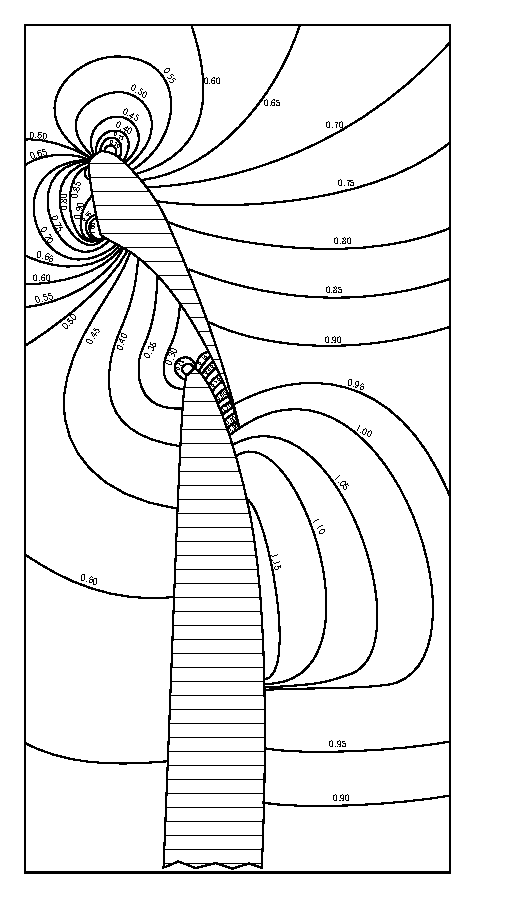
\includegraphics{vol65-figures/fig65-chap7.1.eps}}
\caption{}\label{c6:fig7.1}
\end{figure}

\section{Comments Conclusion}\label{c6:s8}%Sec 8

The methods\pageoriginale that we have described above seem effective for computing 
transonic flows on complicated domains since finite elements 
approximations are used. Moreover the non-linear programming approach 
that we have used (based on an optimal control formulation) gives much 
flexibility for taking into account the \textit{entropy condition} and 
for the choice of the iterative methods for solving the approximate 
problem. We have to observe that regularization method of 
Sec.~\ref{c6:sss5.3.1} is actually a method for computing those 
solutions such that         
\begin{equation}
(\Delta \Phi)^+ \in L^2 (\Omega). \tag{8.1}\label{c6:eq8.1}
\end{equation}
If one wishes to approximate \eqref{c6:eq3.7}, i.e. 
\begin{equation}
(\Delta \Phi)^+ \in L^\infty (\Omega), \tag{8.2}\label{c6:eq8.2}
\end{equation}
one may use a regularization functional like 
\begin{equation}
\int_\Omega \in (x) | (\Delta \phi)^+ |^p dx, p ~\text{``large''}. 
\tag{8.3}\label{c6:eq8.3} 
\end{equation}
All these methods can be extended to 3-dimensional computations, but 
one of the main difficulties is then the treatment of the Kutta - 
Joukowsky condition. For more details and numerical experiments, and 
other methods for treating the entropy condition we refer to GLOWINSKI- 
PIRONNEAU [\ref{k55:e1}], BRISTEAU [\ref{k21:e2}], BRISTEAU 
-GLOWINSKI-PERIAUX-\break PERRIER-PIRONNEAU-POIRIER [\ref{k24:e1}],
[\ref{k24:e2}], BRISTEAU - GLOWIN\-SKI- PERIAUX-PERRIER-PIRONNEAU
[\ref{k23:e1}].      

In CEA-GEYMONAT [\ref{k26:e1}] one may find results on the solution of
nonlinear boundary value problems via optimal control.   

Let us mention to conclude that various methods for treating shocks in 
fluid mechanic problems can be found in LASCAUX [\ref{k65:e1}] and the 
bibliography therein.   
